\documentclass[17pt]{beamer}

\usepackage{StyleBeamer}

%\selectcolormodel{cmyk}

%\usepackage{wrapfig}
%\makeatletter
%\setlength{\parskip}{1ex}
%\newcommand{\@minipagerestore}{\setlength{\parskip}{1ex}}

\setbeamertemplate{navigation symbols}{}

% Début du document
%%%%%%%%%%%%%%%%%%%
\begin{document}

\title{Questions flash}
\frame{\titlepage}

\centering
\begin{frame}\frametitle{Question 1}
Développer l'expression $A=5 \times (3x-5)^2$
\end{frame}

\begin{frame}\frametitle{Question 2}
Soient $\vv u \dbinom 3 7$ et $\vv v \dbinom {-2} 1$. Calculer les coordonnées de $\vv u -2 \vv v$.
\end{frame}

\begin{frame}\frametitle{Question 3}
Factoriser l'expression $2(4x+3)-5x(4x+3)$.
\end{frame}

\begin{frame}\frametitle{Question 4}\setlength{\composep}{3pt}
\compo[0.5]
{
\small On se donne le tableau de signes d'une fonction $f$. Quelle courbe parmi $\mathscr C_1$ et $\mathscr C_2$ représente $f$?
}
{
\resizebox{\linewidth}{!}{
\begin{tikzpicture}
\tkzTabInit[lgt=1.3,espcl=1.2,deltacl=0.4]{$x$/1, $f(x)$/1}{1,3,8,12}
\tkzTabLine{,+,z,-,z,+,}
\end{tikzpicture}}
}

\begin{center}
\begin{tikzpicture}
\begin{axis}[
styleglobal,
width=0.9*\linewidth,
xmin=-1.5, xmax=13.5,
ymin=-2.5, ymax=3.5,
xtick distance=1,
ytick distance=1,
minor x tick num=1,
minor y tick num=1,
grid style={dash pattern=on 2.4pt off 1.6pt,line width=0.64pt,draw=black!35},
minor grid style={line width=0.4pt,draw=black!20},
]
\addplot[styleplot,domain=(0:8),tension=0.7] plot coordinates {(1,2) (3,0) (5,-2) (8,0) (12,1)} node[pos=0.75,above left] {$\mathscr C_1$} \pointsextremites;
\addplot[styleplot,color=red!50!black,densely dashed,tension=0.2] plot coordinates{(1,-1) (3,0) (5,-1) (8,-2) (12,2)} node[pos=0.7,below right] {$\mathscr C_2$} \pointsextremites;
\end{axis}
\end{tikzpicture}
\end{center}

\end{frame}
\end{document}
